\chapter{Results}
\label{ch:Results}
We successfully showed that the method of attention based selection can be used with other log parsing algorithms and that it improves the prediction quality for some datasets, but not all. Additionally, we show that for small datasets, removing timestamps greatly increased the prediction quality. 

\section{Influence of Timestamps}
\label{sec:Results:Timestamps}
We evaluated the prediction performance of our ML pipeline on three different dataset sizes. The data shows a strong improvement for small dataset sizes that shrinks with increasing dataset size. The prediction quality without timestamps is always superior compared to the experiments run with timestamps. When using attention based selection, the variance is already much lower compared to fixed parameter templates with timestamps. We named the full dataset 200k logs, but in reality the full log size was only 169k logs. We stuck with it for the naming scheme, but the exact size is not as important as the order of magnitude in comparison to the smaller sets. 

\begin{figure}[H]
    \centering
    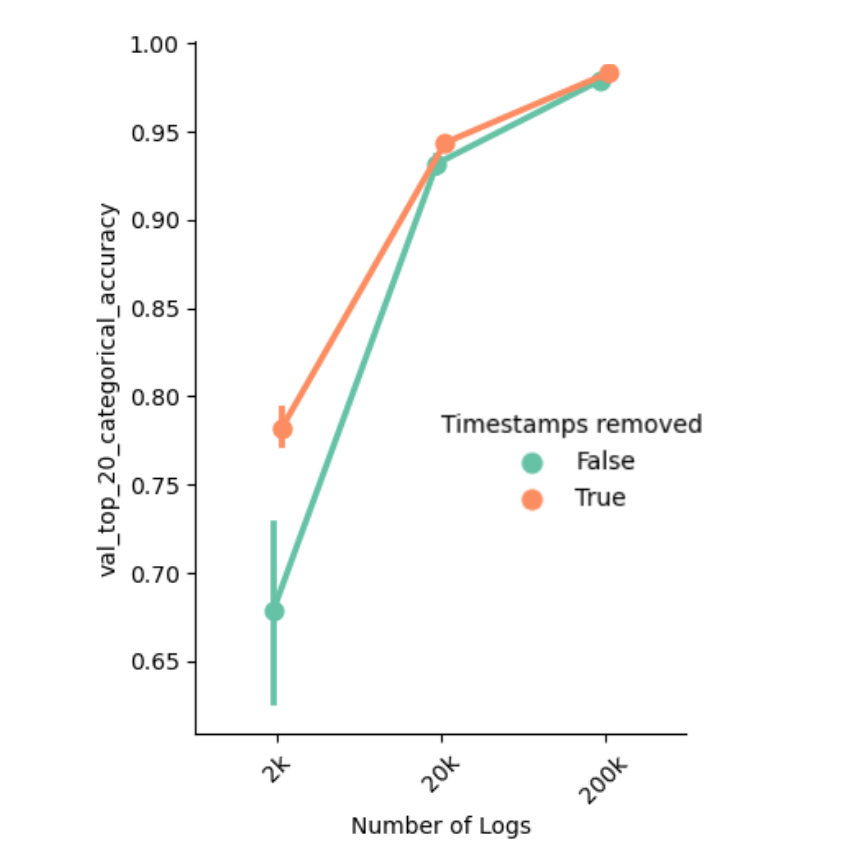
\includegraphics[keepaspectratio=true,scale=0.8]{figures/5_results/timestamps_comparison.png}
    \caption{Two line plots showing the prediction quality at different dataset sizes, with and without timestamps.}
    \label{fig:TimestampsComparison}
\end{figure}

When we look at the particular results for the biggest dataset, we can see that removing timestamps decreases variance of prediction quality across all fixed parameter templates. Finer granularity templates especially benefit from removing timestamps. 
\begin{figure}[H]
    \centering
    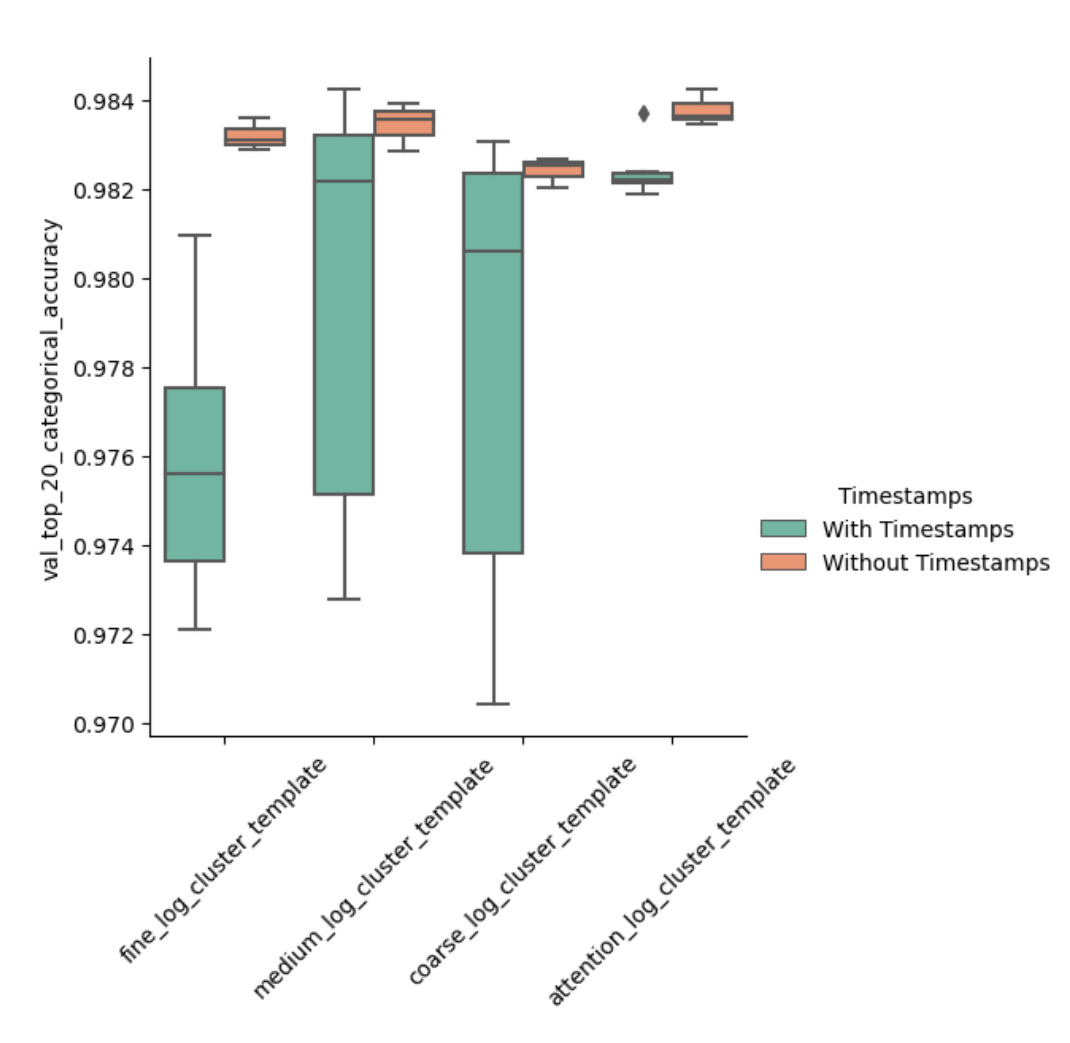
\includegraphics[keepaspectratio=true,scale=0.8]{figures/5_results/Timestamps_templates.png}
    \caption{The effect of timestamps on different levels of log template granularity and attention based selection. Dataset size 200k logs.}
    \label{fig:TimestampsTemplates}
\end{figure}

As can be seen in table \ref{tab:runtimes}, running the experiments with and without timestamps took approximately the same time for all dataset sizes. 
\begin{table}[htbp]
  \centering
  \begin{tabular}{ccc}
    \hline
    \textbf{Dataset Size} & \textbf{Runtime (With Timestamps)} & \textbf{Runtime (Without Timestamps)} \\
    \hline
    200k & 21.6 min & 22 min \\
    20k & 3.7 min & 3.7 min \\
    2k & 1.3 min & 1.3 min \\
        \hline

  \end{tabular}
    \caption{Runtime comparison with and without timestamps for different dataset sizes}
      \label{tab:runtimes}

\end{table}


\section{Individual Algorithms}
\label{sec:Results:Algos}
The attention mechanism, illustrated in figure \ref{fig:results:Algos}, delivered very good results, especially for Nulog and Spell, where it lead to the highest median accuracy of ~0.83 and ~0.84 respectively. Additionally, the data shows that not one type of granularity is best for each algorithm. Drain and Nulog benefited from more "finer" parameterization, while for Spell the "medium" settings lead to the best results, bar attention based selection. Overall, the results between the different log parsing algorithms are very similar at this dataset size. 

\begin{figure}[H]
     \centering
     \begin{subfigure}[b]{0.45\textwidth}
         \centering
        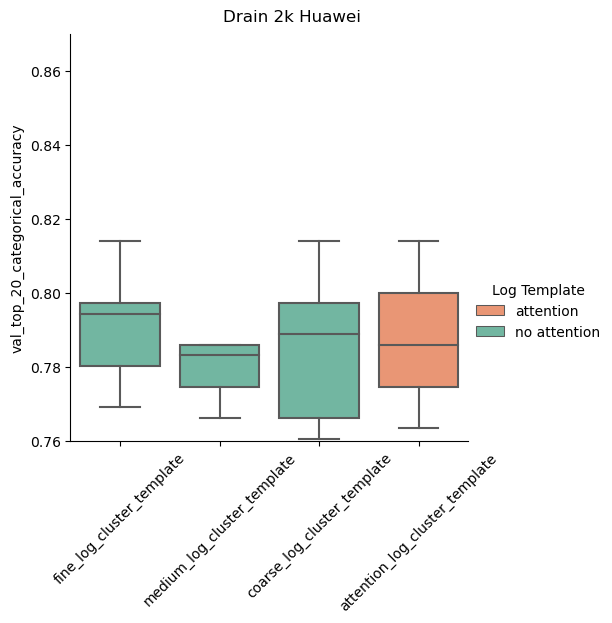
\includegraphics[keepaspectratio=true,scale=0.45]{figures/5_results/Drain_Huawei_2k.png}
         \caption{Drain}
         \label{fig:results:drain}
     \end{subfigure}
     \hfill
     \begin{subfigure}[b]{0.45\textwidth}
         \centering
        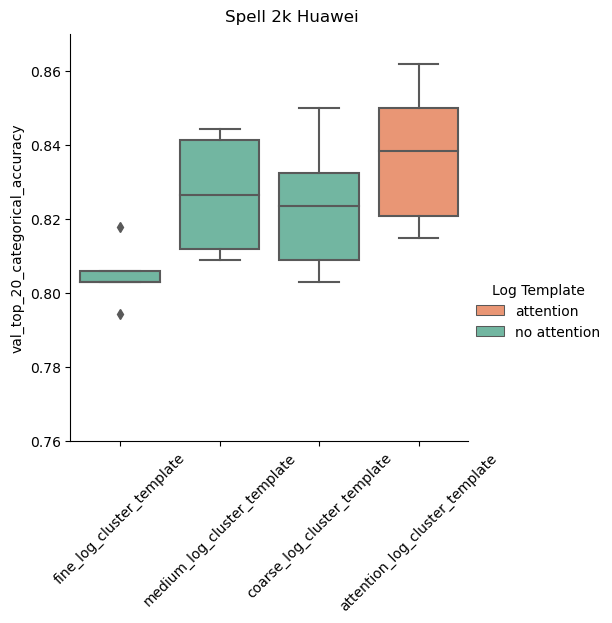
\includegraphics[keepaspectratio=true,scale=0.45]{figures/5_results/Spell_Huawei_2k.png}
         \caption{Spell}
         \label{fig:results:spell}
     \end{subfigure}
     \hfill
     \begin{subfigure}[b]{0.45\textwidth}
         \centering
        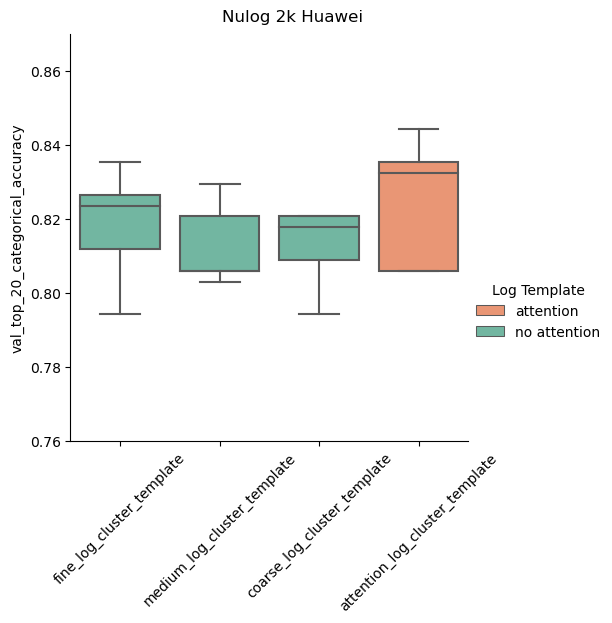
\includegraphics[keepaspectratio=true,scale=0.45]{figures/5_results/Nulog_Huawei_2k.png}
         \caption{Nulog}
         \label{results:nulog}
     \end{subfigure}
        \caption{Three plots comparing attention based selection to fixed parameter template baseline for Drain, Spell and Nulog. Dataset size 2000 logs. }
        \label{fig:results:Algos}
\end{figure}

With 2000 logs, the training time for our model is around 1.5 minutes for Spell and Drain and 3.5minutes for Nulog. Attention based selection had no impact on runtime at this dataset size. 

As can be seen in \ref{tab:log_parsers_comparison}, changing the parameters of the log parsers has great influence on the number of templates. Drain especially produces much more templates than the other two algorithms, which will become more obvious in the Thunderbird dataset.  

\begin{table}[htbp]
  \centering
  \begin{tabular}{ccccc}
    \hline
    \textbf{Parser} & \textbf{Fine} & \textbf{Medium} & \textbf{Coarse} & \textbf{Attention} \\
    \hline
    Drain & 198 & 174 & 154 & 526 \\
    Spell & 172 & 117 & 85 & 374 \\
    Nulog & 106 & 123 & 133 & 363 \\
    \hline
  \end{tabular}
  \caption{Effect of log parser parameterization on median number of generated log templates. Median values. Attention is the sum of the other three types of templates. Dataset size 2000 logs.}
  \label{tab:log_parsers_comparison}
\end{table}

\section{Combining multiple algorithms}
\label{sec:Results:Combination}
\subsection{All Algorithms}
When combining the templates generated by our log parsing algorithms Drain, Spell and Nulog and feeding it into the attention mechanism, the results are not as clear as with the individual parsers. While the difference in quality is lower, the attention mechanism still selected templates that led to the highest median accuracy of ~0.822. We observe that this value is slightly lower compared to using just Spell or Nulog. The runtime when using the templates generated by all log parsing algorithms is very similar compared to using only Nulog.

% Talked about runtime, template number is obvious?, quality. What else can I say here?

\begin{figure}[H]
    \centering
    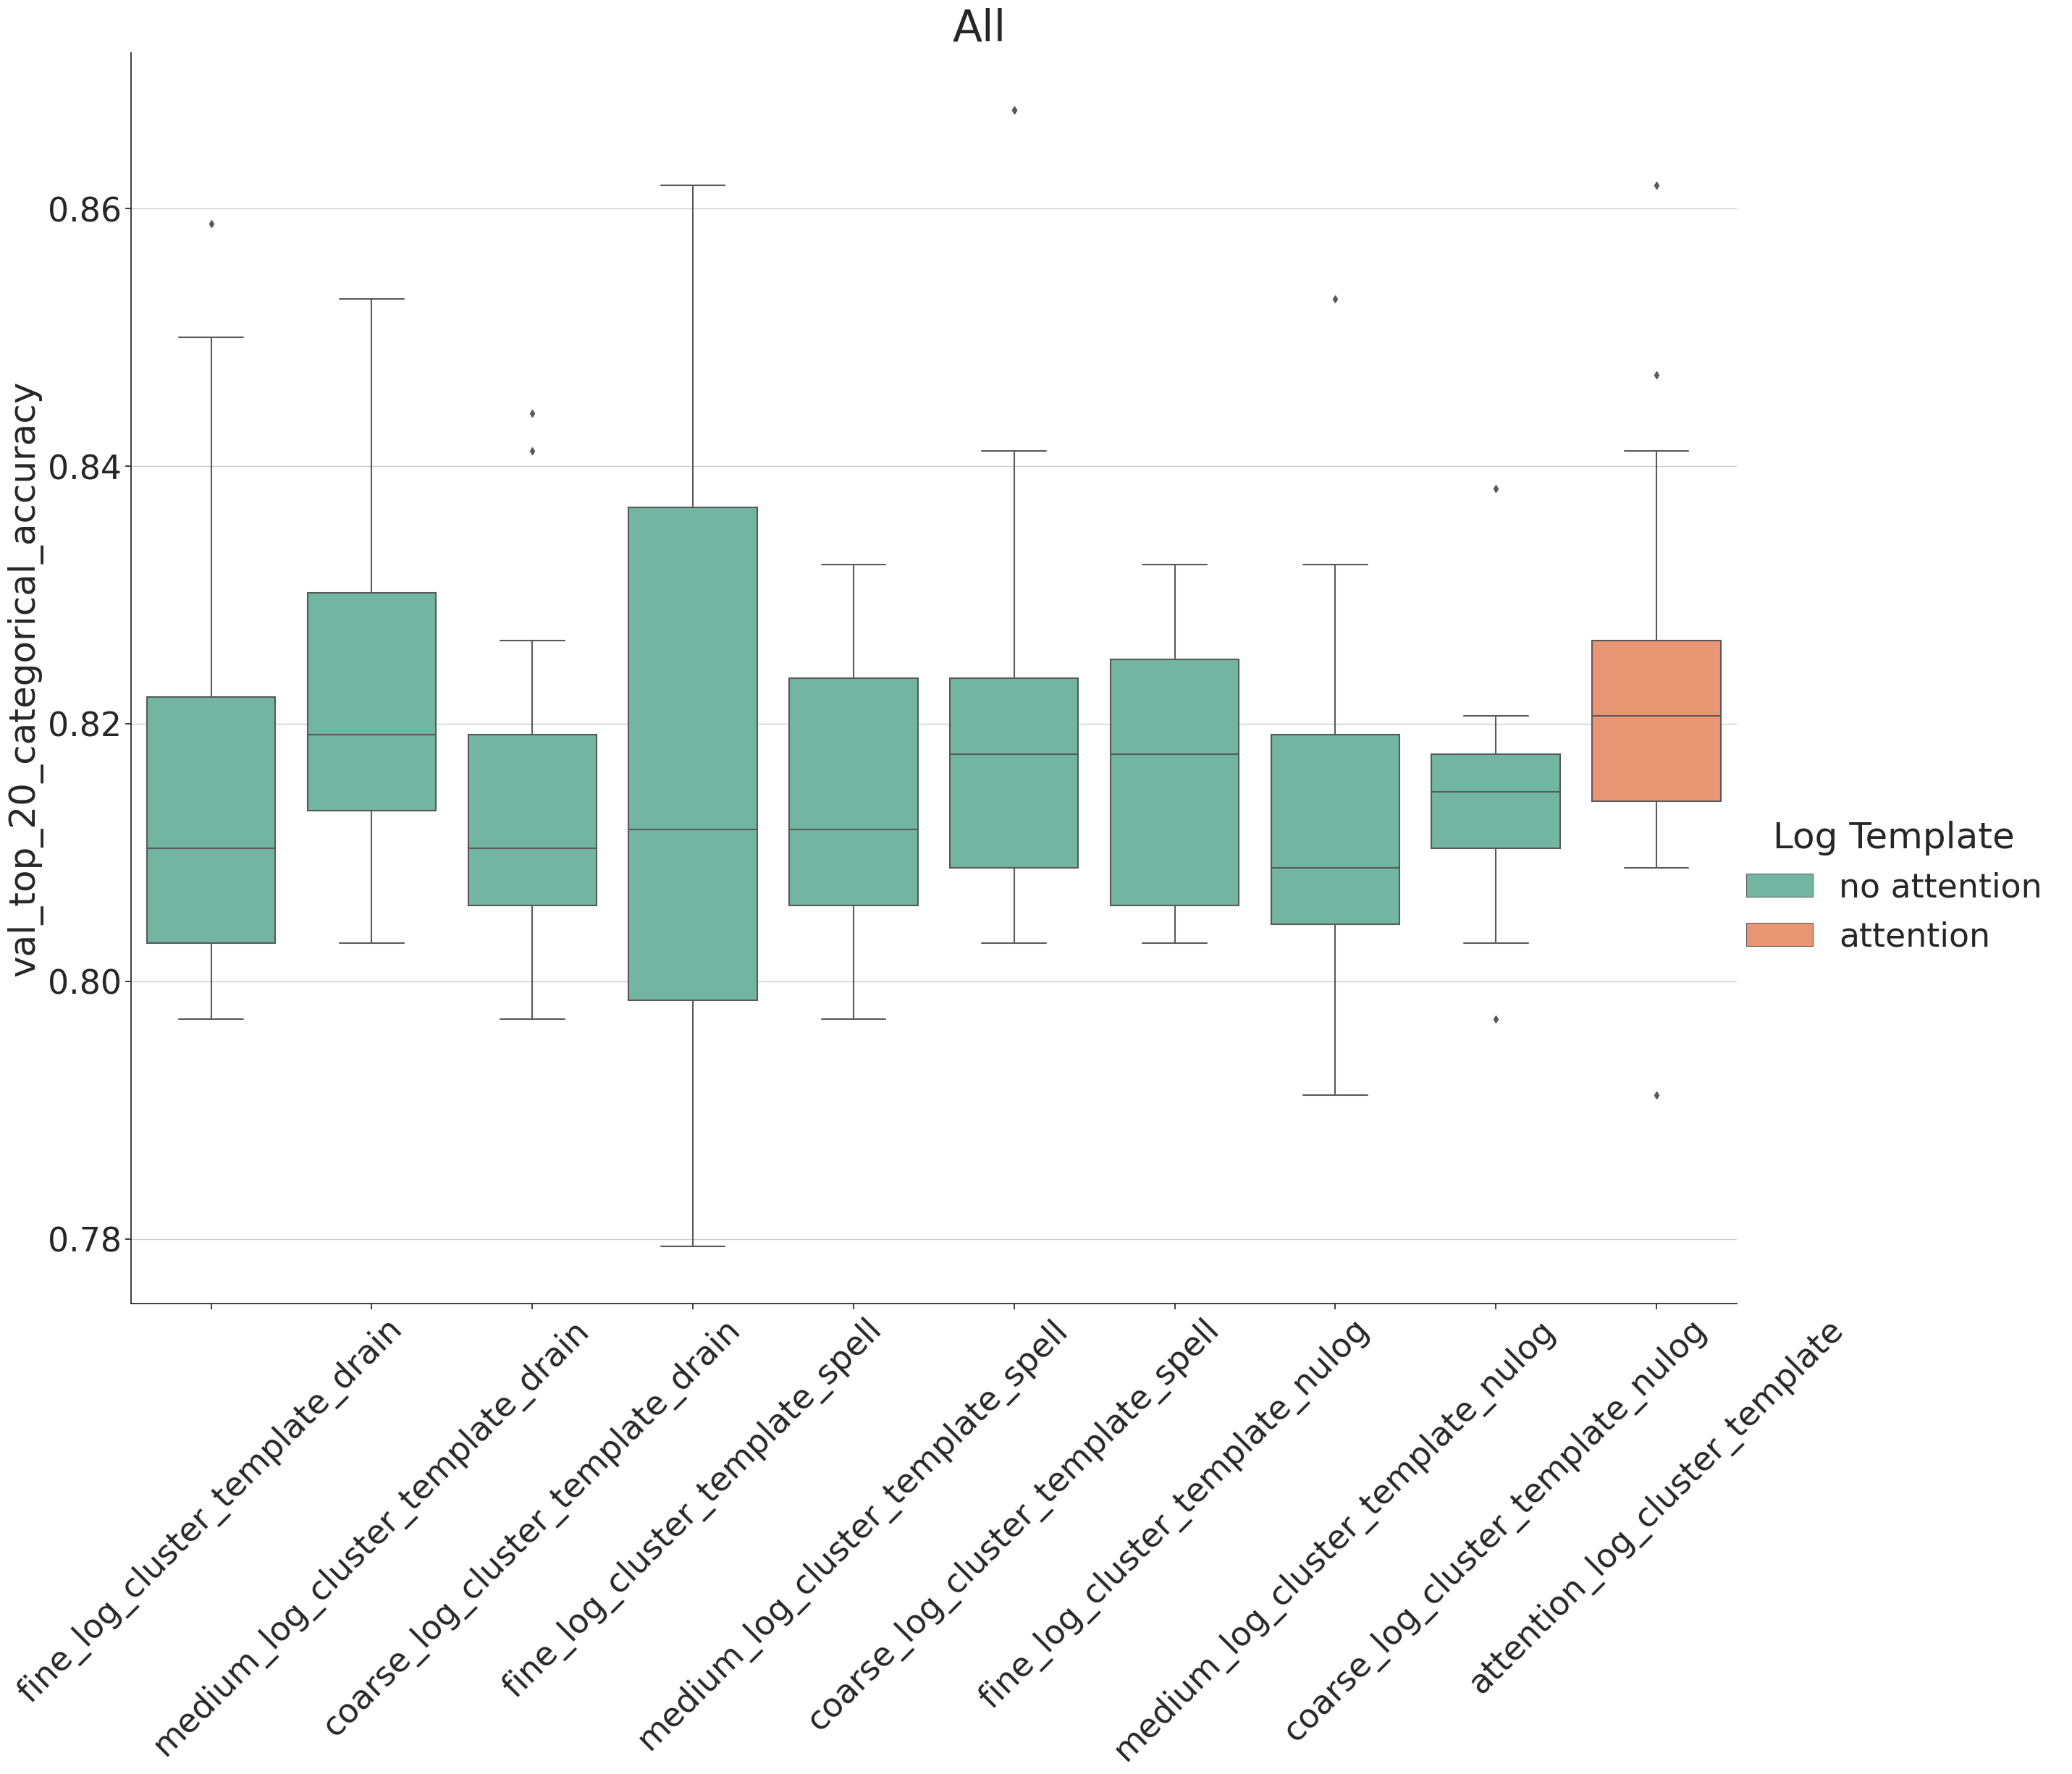
\includegraphics[keepaspectratio=true,scale=0.15]{figures/5_results/All_Huawei_2k.png}
    \caption{Attention based selection from nine log templates generated by three log parsers with three parameterizations. Dataset size 2000 logs.}
    \label{fig:all_together}
\end{figure}

\begin{table}[htbp]
  \centering

  \begin{tabular}{c c}
    \hline
    \textbf{Parser} & \textbf{Runtime} \\
    \hline
    Drain & 1.3 min \\
    Nulog & 4.1 min \\
    Spell & 1.2 min \\
    All & 4.2 min \\
    \hline
  \end{tabular}
    \caption{Runtime Comparison of Log Parsers}
  \label{tab:log_parsers_runtime}
\end{table}

\subsection{Combination of individual algorithms}
\label{sec:Results:Mixing}
We not only ran experiments using all log parsing algorithms at once, but also did tests with all possible combinations of two out three parsers. We can see in every figure, that no combination of log parsers resulted in a definite improvement compared to baseline as observed in the experiments using only a single log parsing algorithm. Interestingly, combining Drain and Spell led to better results than using all algorithms, as can be seen in figure \ref{fig:drain_spell}. The median accuracy with attention based selection in this experiment was ~0.835, compared to ~0.822 in figure \ref{fig:all_together}.

\begin{figure}[H]
    \centering
    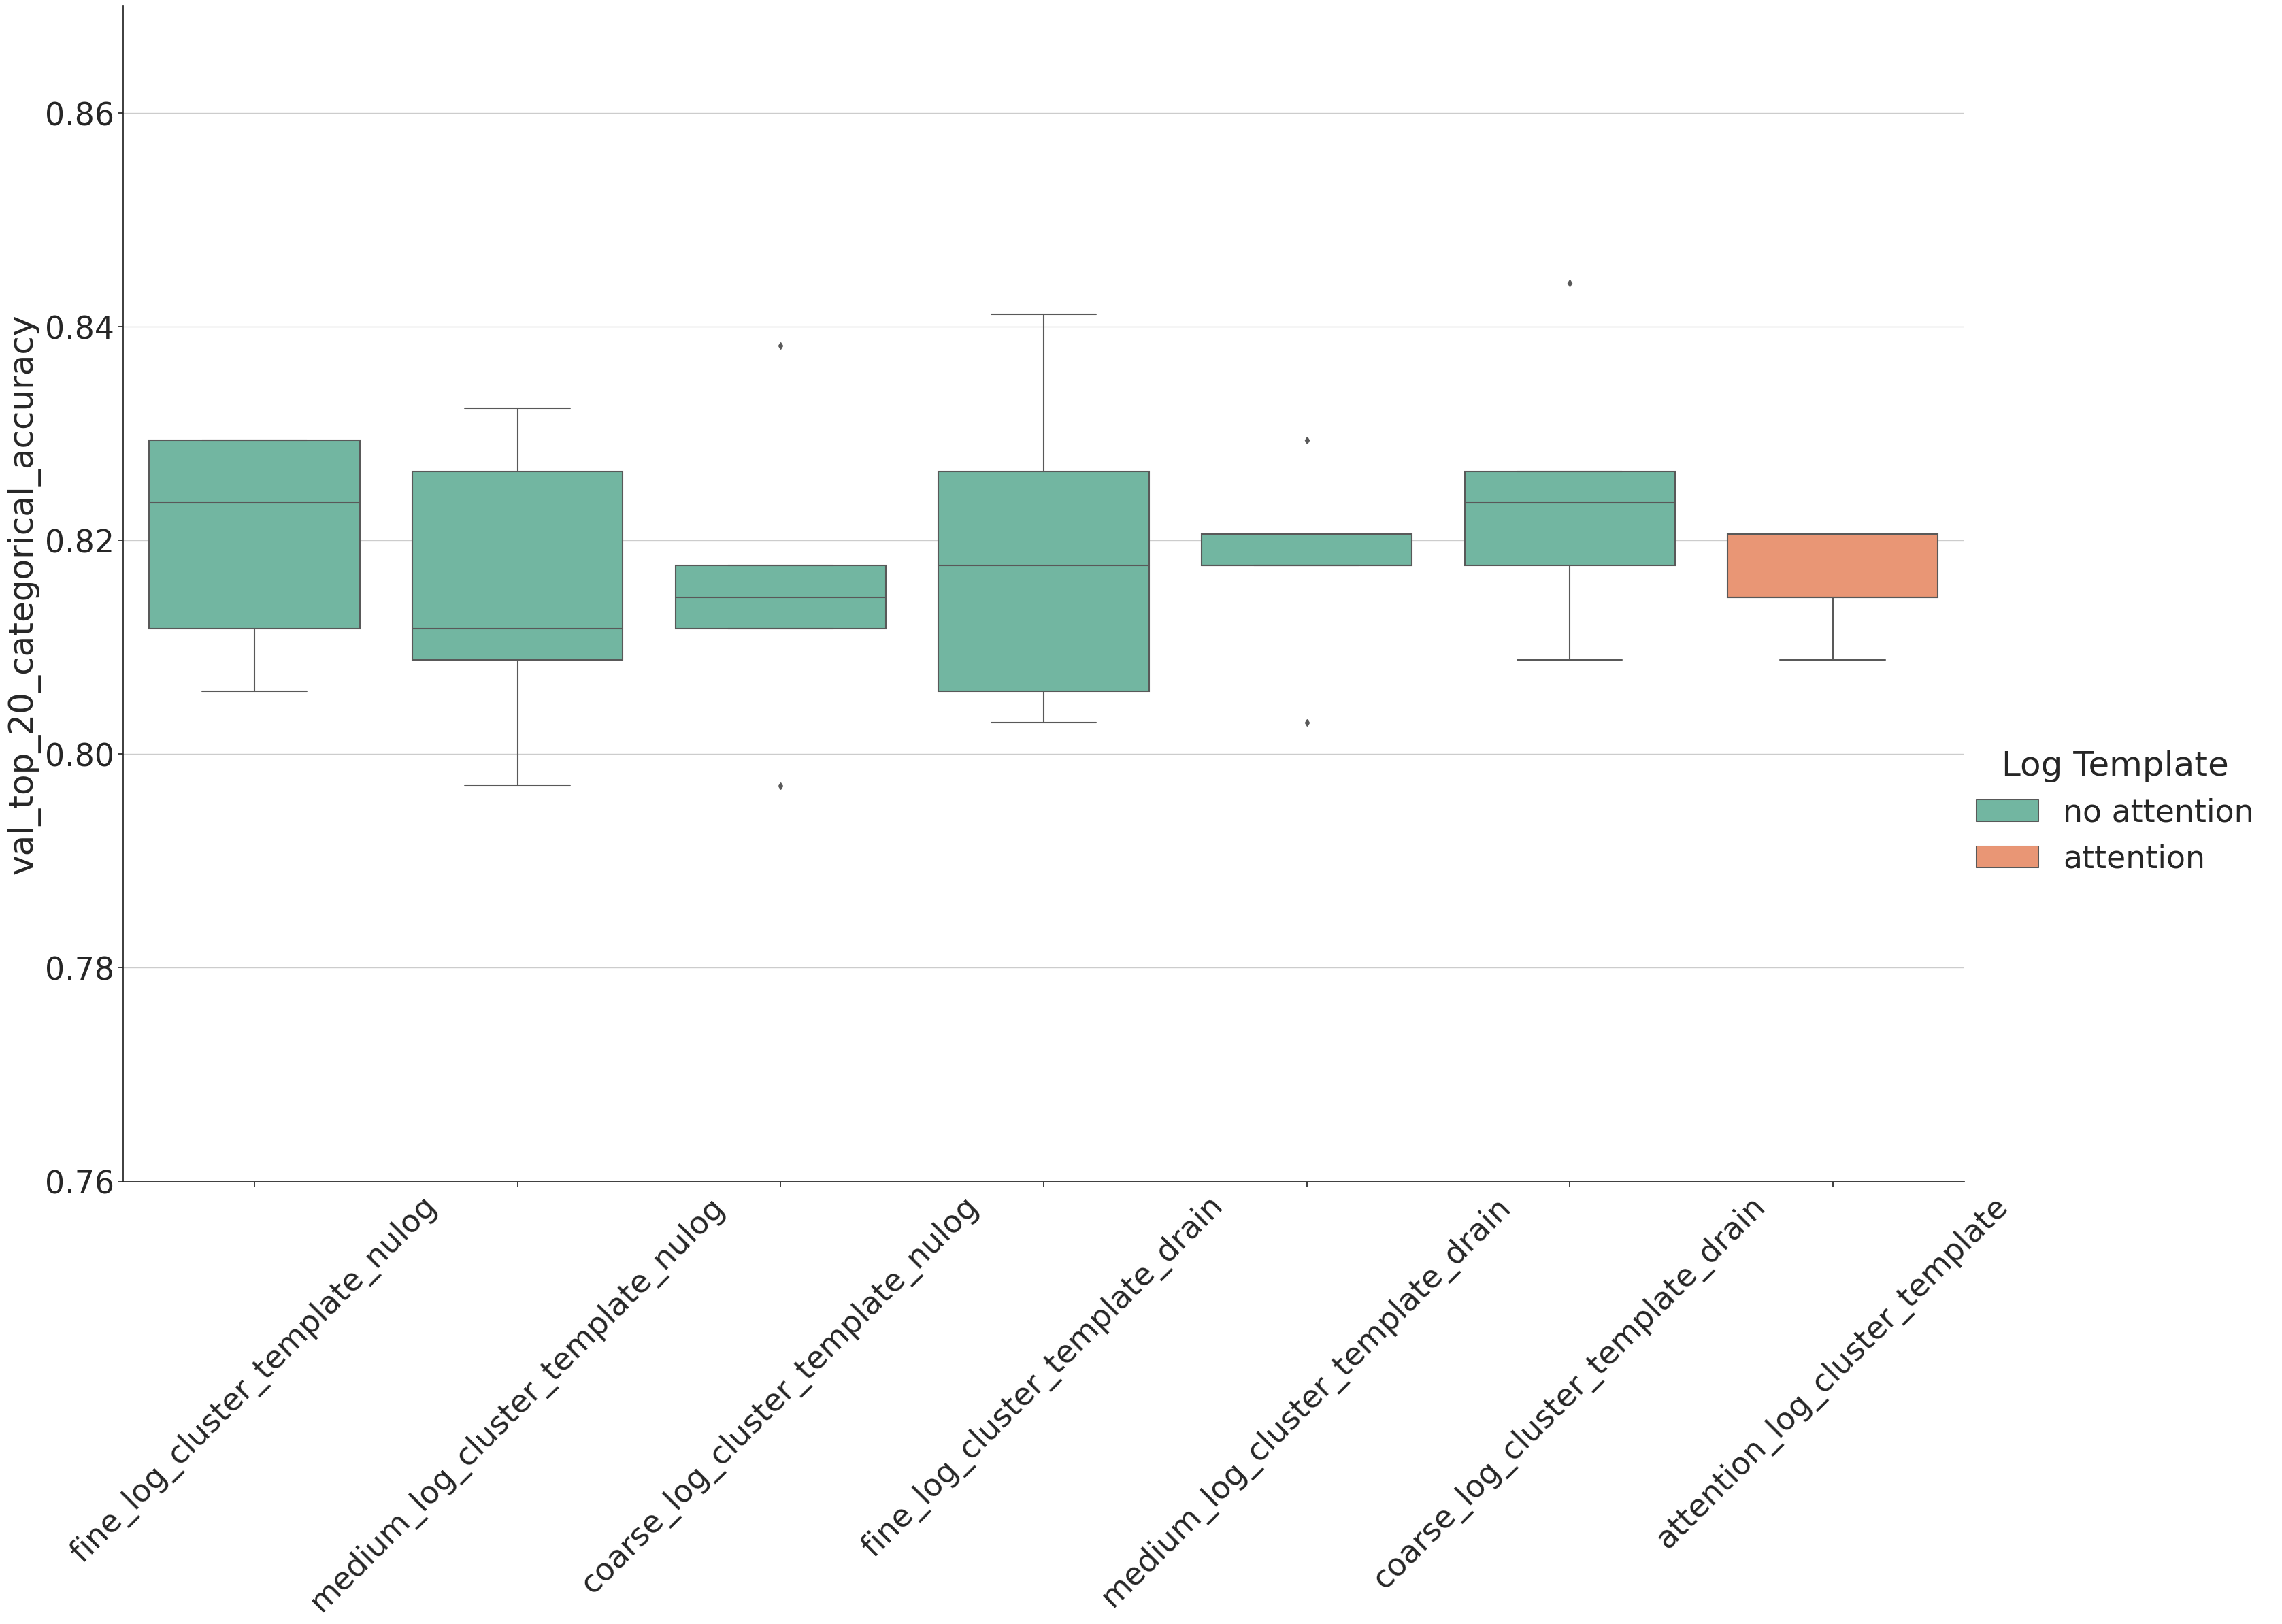
\includegraphics[keepaspectratio=true,scale=0.15]{figures/5_results/drain+nulog.png}
    \caption{Attention based selection from log templates generated Nulog and Drain. Dataset size 2000 logs.}
    \label{fig:drain_nulog}
\end{figure}

\begin{figure}[H]
    \centering
    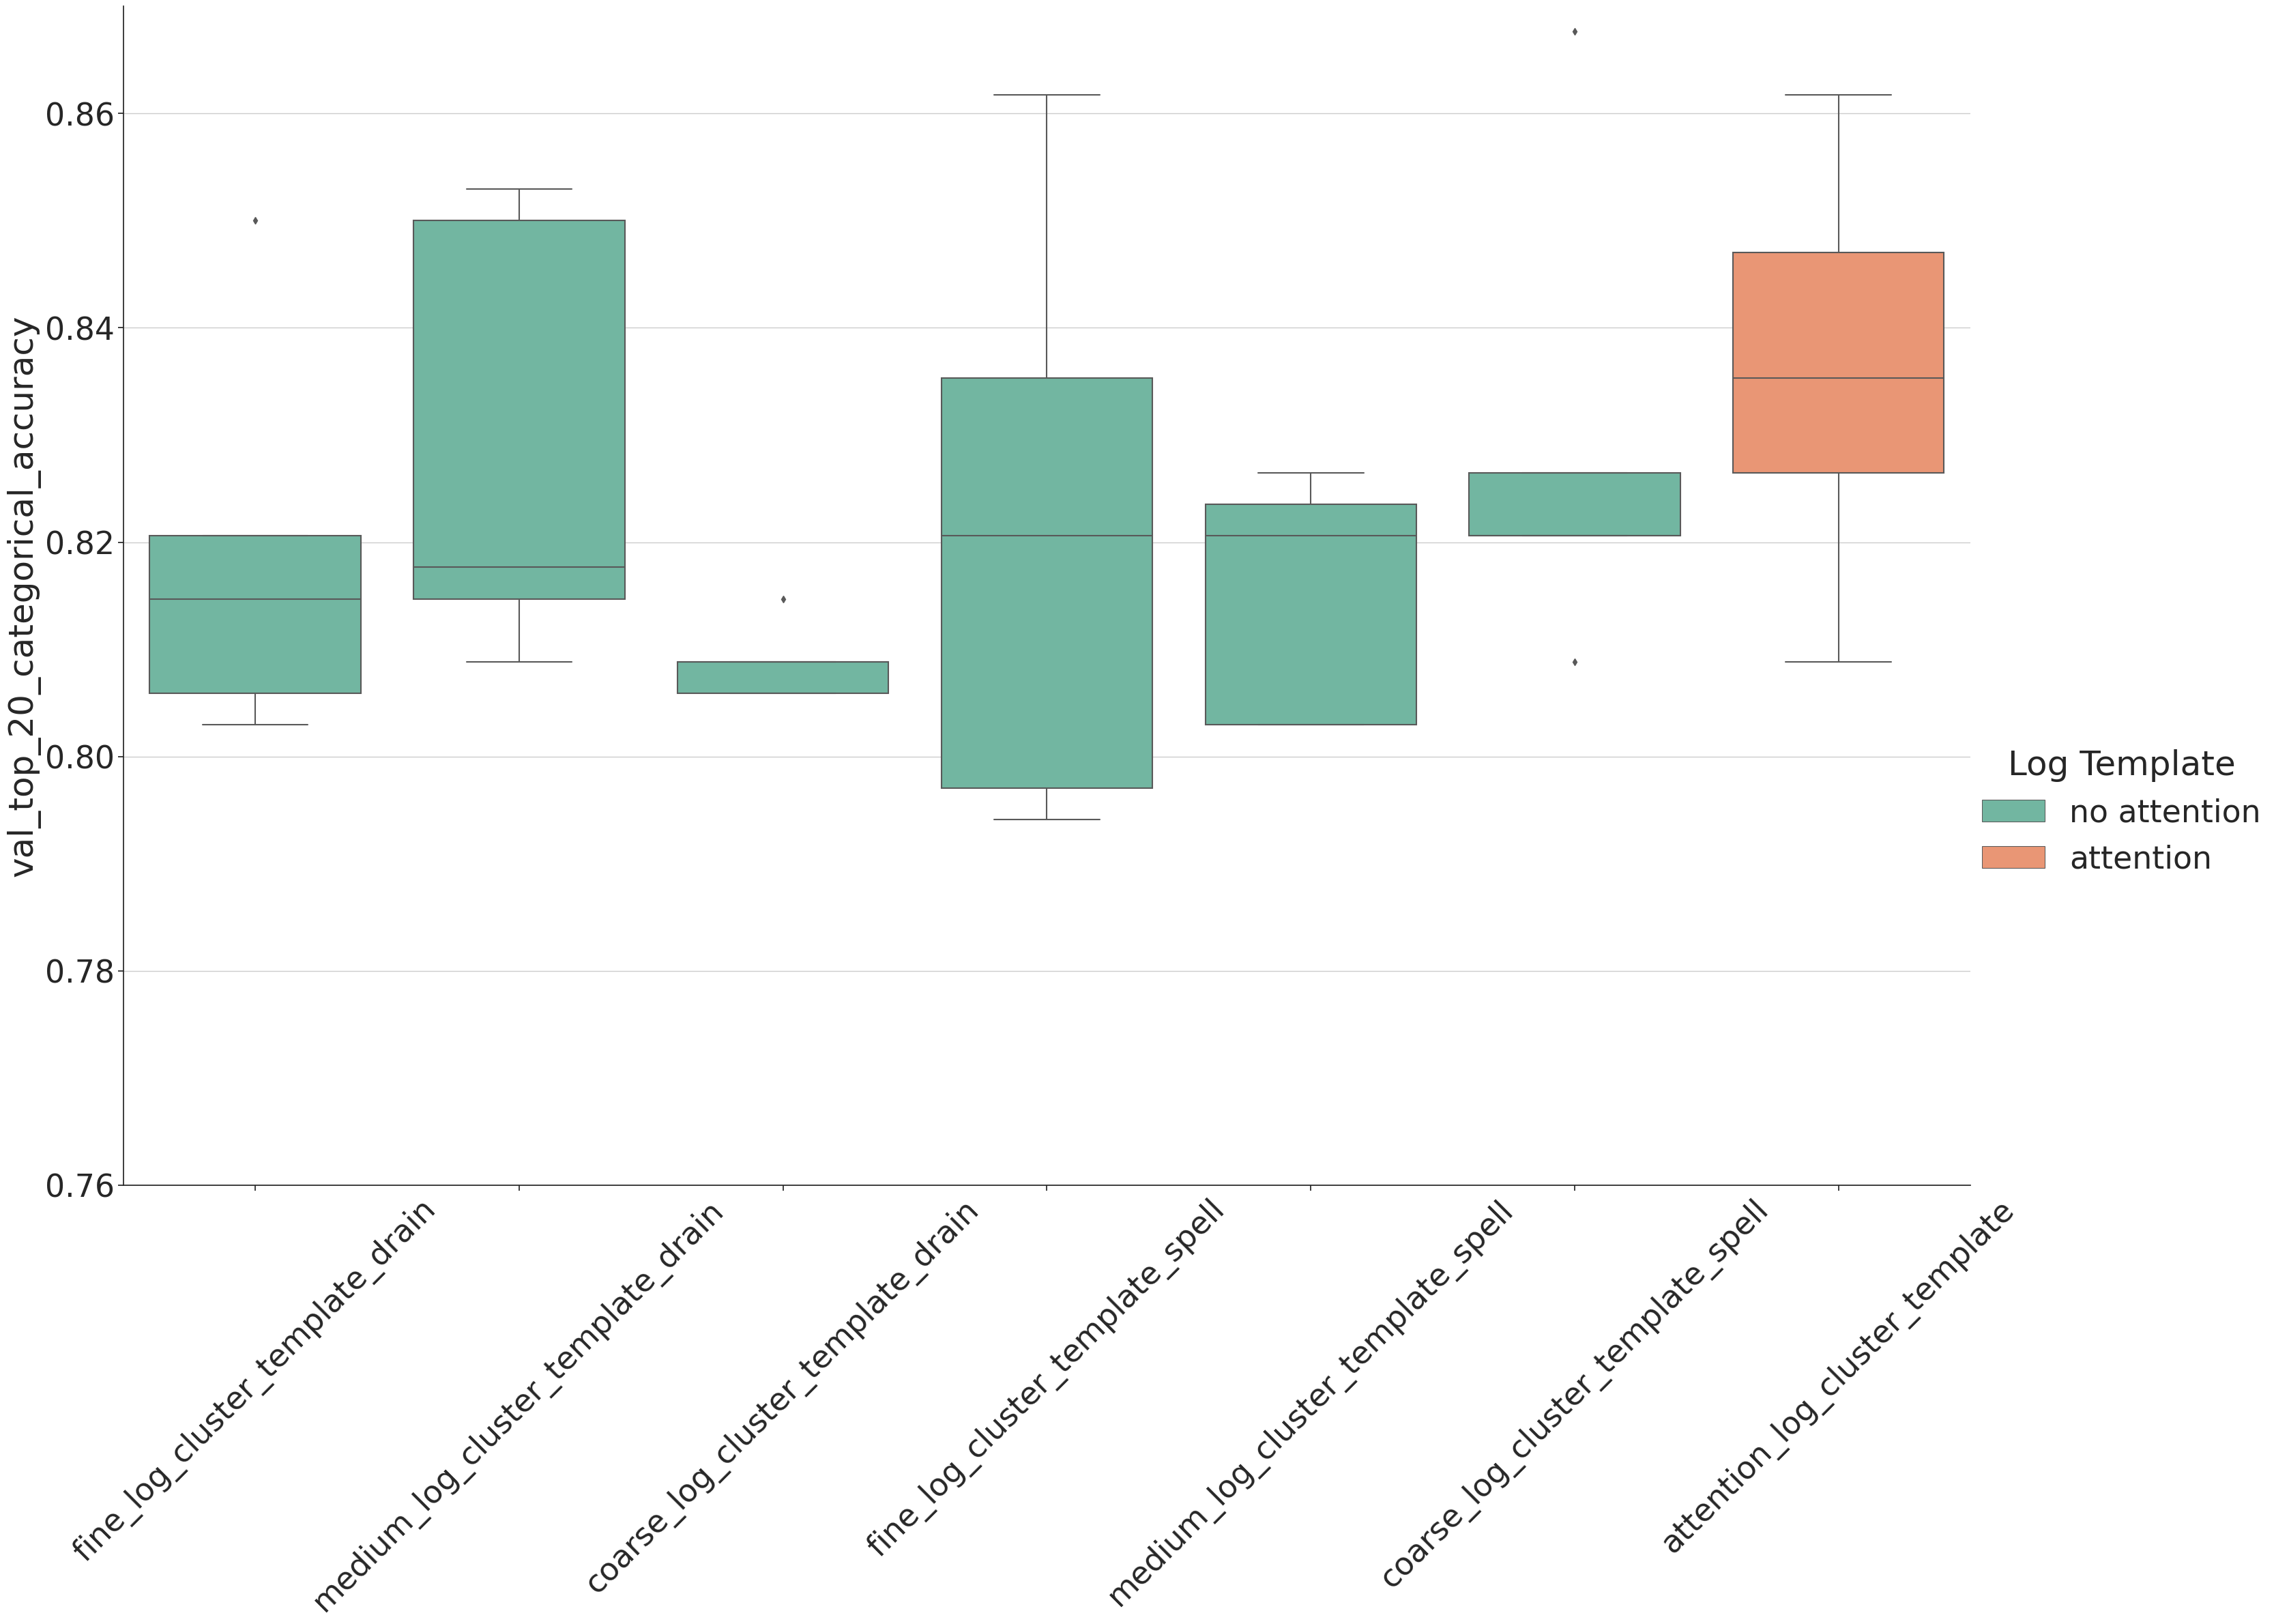
\includegraphics[keepaspectratio=true,scale=0.15]{figures/5_results/drain+spell.png}
    \caption{Attention based selection from log templates generated by Spell and Drain. Dataset size 2000 logs.}
    \label{fig:drain_spell}
\end{figure}

\begin{figure}[H]
    \centering
    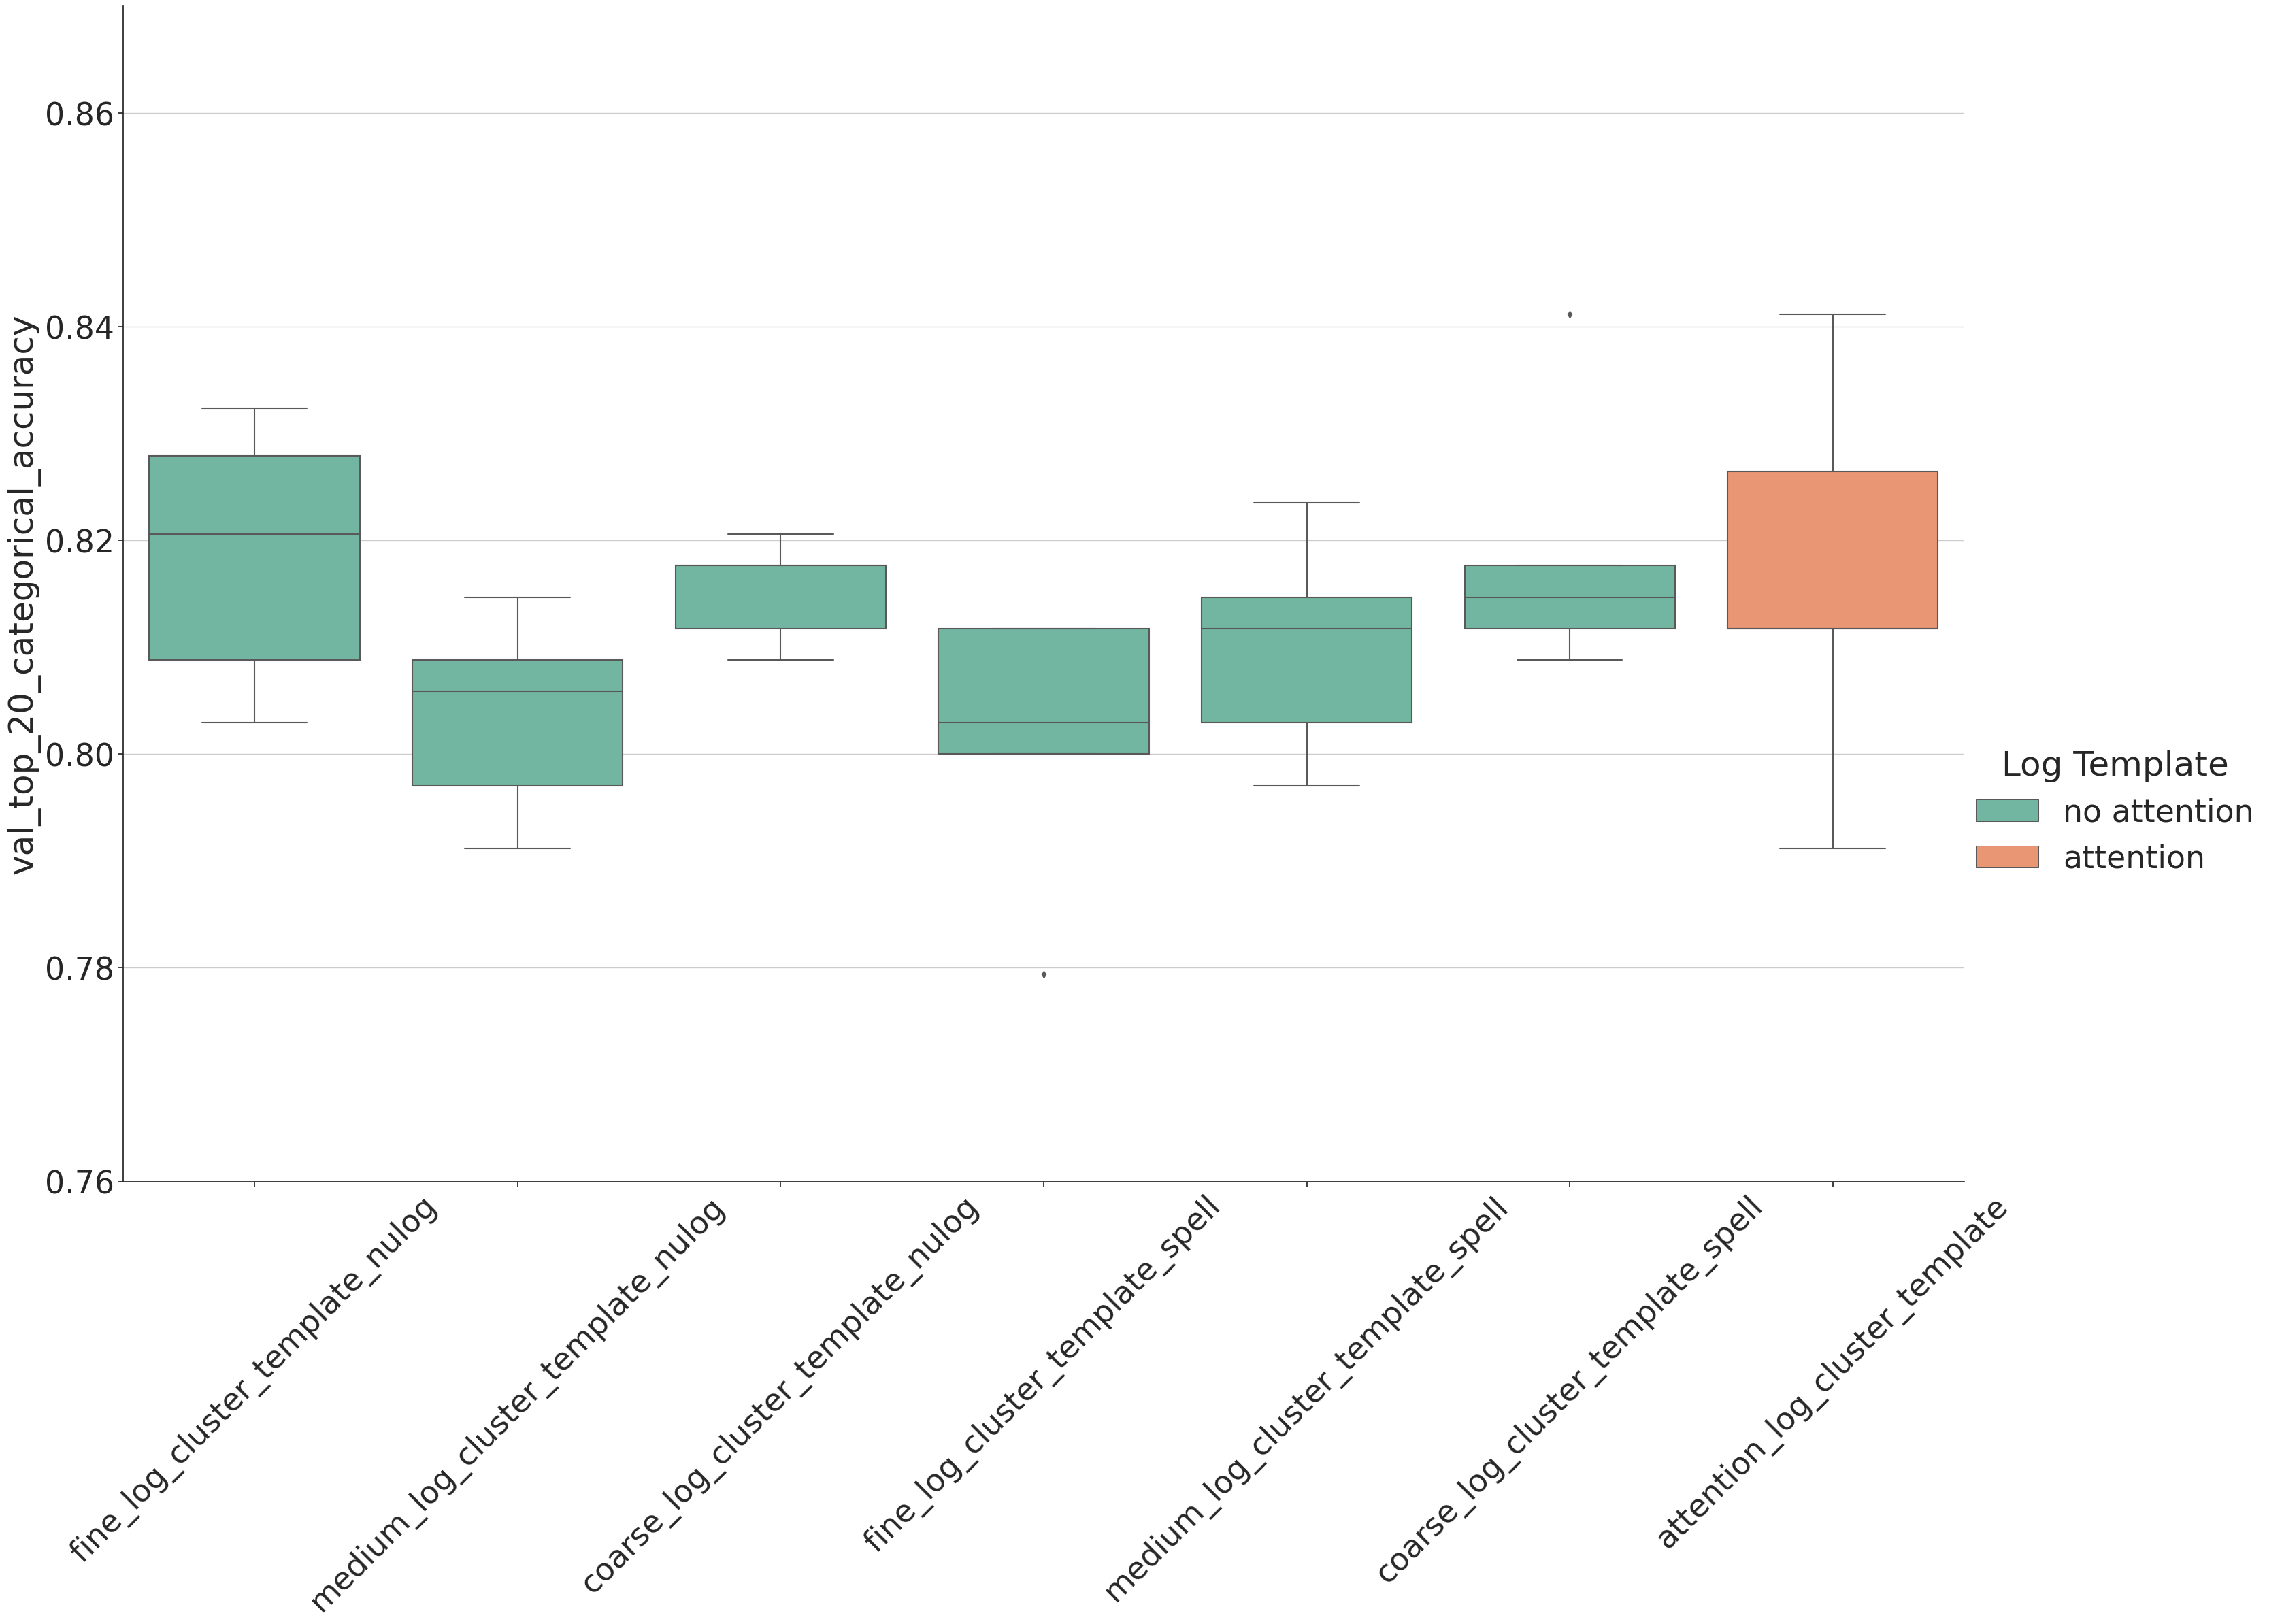
\includegraphics[keepaspectratio=true,scale=0.15]{figures/5_results/nulog+spell.png}
    \caption{Attention based selection from log templates generated by Nulog and Spell. Dataset size 2000 logs.}
    \label{fig:nulog_spell}
\end{figure}




\section{Other Datasets}
We repeated some of the experiments conducted with the original dataset with two other datasets, in particular, we evaluated the attention based selection of log templates generated by the individual algorithms and by a combination of all of them.

\subsection{HDFS}
On the HDFS dataset, we observed various differences compared to our experiments on the original logs. We can see in table \ref{tab:hdfs} that the number of templates generated by Drain is almost ten times higher compared to Nulog and Spell, which were much closer to each other for the original dataset. Furthermore, our model trained for much shorter than the 25 epochs that we set, which was also not the case with our previous experiment. The total runtime stayed very similar.  

\begin{table}[htbp]
  \centering
  \begin{tabular}{cccc}
    \hline
    \textbf{Parser} & \textbf{No. of Templates} & \textbf{Runtime} & \textbf{Epochs learned} \\
    \hline
    Drain & 441  & 1.8min & 9 \\
    Spell & 57   & 1.9min & 10 \\
    Nulog & 54  & 4.6min & 16 \\
    All & 553 & 4.7min & 16 \\
    \hline
  \end{tabular}
  \caption{Number of log templates, epochs learned and runtime for different log parsers. HDFS logs.}
  \label{tab:hdfs}
\end{table}

Figure \ref{fig:results:hdfs} shows the results for the individual log parsing algorithms, similar to figure \ref{fig:results:Algos}. We can see that the overall prediction quality is slightly worse and that Nulog performs best again. For all algorithms the templates selected by the attention mechanism do not lead to a better result, but in all cases the medium parameters delivered the best prediction quality. 

\begin{figure}[H]
     \centering
     \begin{subfigure}[b]{0.45\textwidth}
         \centering
        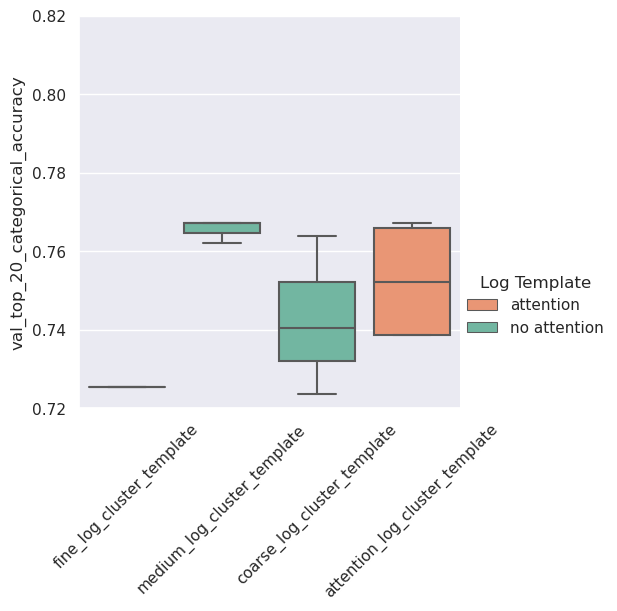
\includegraphics[keepaspectratio=true,scale=0.45]{figures/5_results/drain_hdfs.png}
         \caption{Drain}
         \label{fig:results:drain_hdfs}
     \end{subfigure}
     \hfill
     \begin{subfigure}[b]{0.45\textwidth}
         \centering
        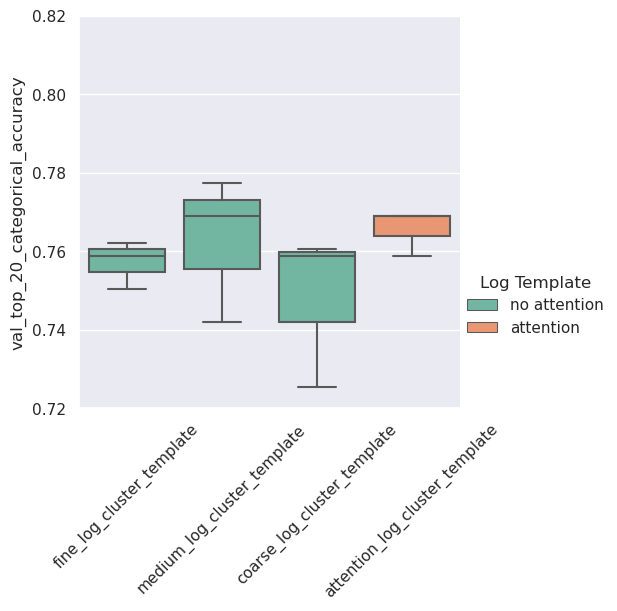
\includegraphics[keepaspectratio=true,scale=0.45]{figures/5_results/spell_hdfs.png}
         \caption{Spell}
         \label{fig:results:spell_hdfs}
     \end{subfigure}
     \hfill
     \begin{subfigure}[b]{0.45\textwidth}
         \centering
        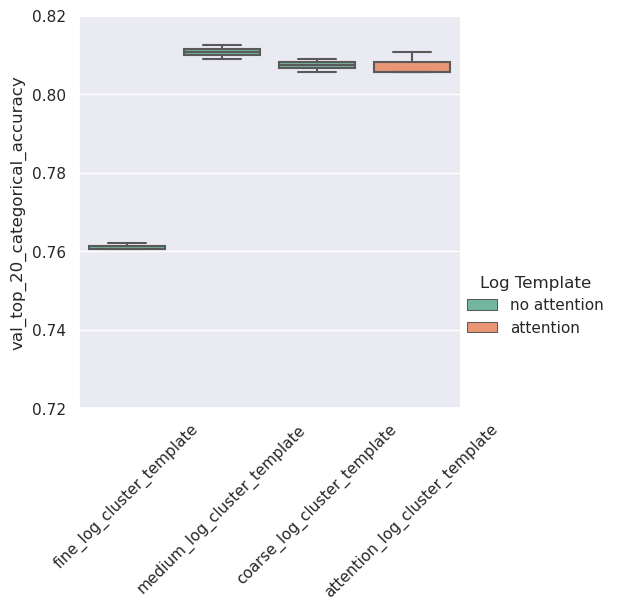
\includegraphics[keepaspectratio=true,scale=0.45]{figures/5_results/nulog_hdfs.png}
         \caption{Nulog}
         \label{results:nulog_hdfs}
     \end{subfigure}
        \caption{Three plots comparing attention based selection to fixed parameter template baseline for Drain, Spell and Nulog. Dataset size 2000 logs. }
        \label{fig:results:hdfs}
\end{figure}

Figure \ref{fig:average_hdfs} shows the average prediction quality of all individual log parsers. We can see here that  attention selected templates lead to a higher median accuracy, but that this improvement is very small. 

\begin{figure}[H]
    \centering
    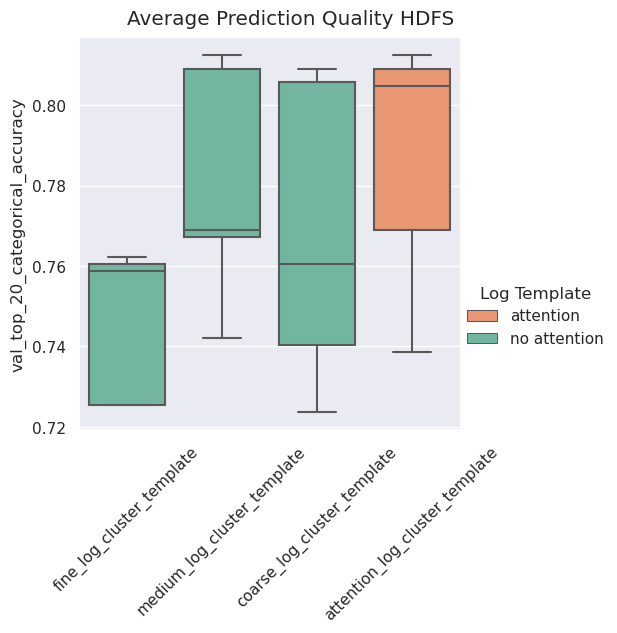
\includegraphics[keepaspectratio=true,scale=0.6]{figures/5_results/average_hdfs.png}
    \caption{Average prediction quality over all log parsing algorithms. Dataset size 2000 logs.}
    \label{fig:average_hdfs}
\end{figure}

When feeding all the templates from all our parsers into the attention mechanism, we observe that the attention results are very good and on par with the Nulog results, but are not the best overall as can be seen in figure \ref{fig:all_hdfs}.
\begin{figure}[H]
    \centering
    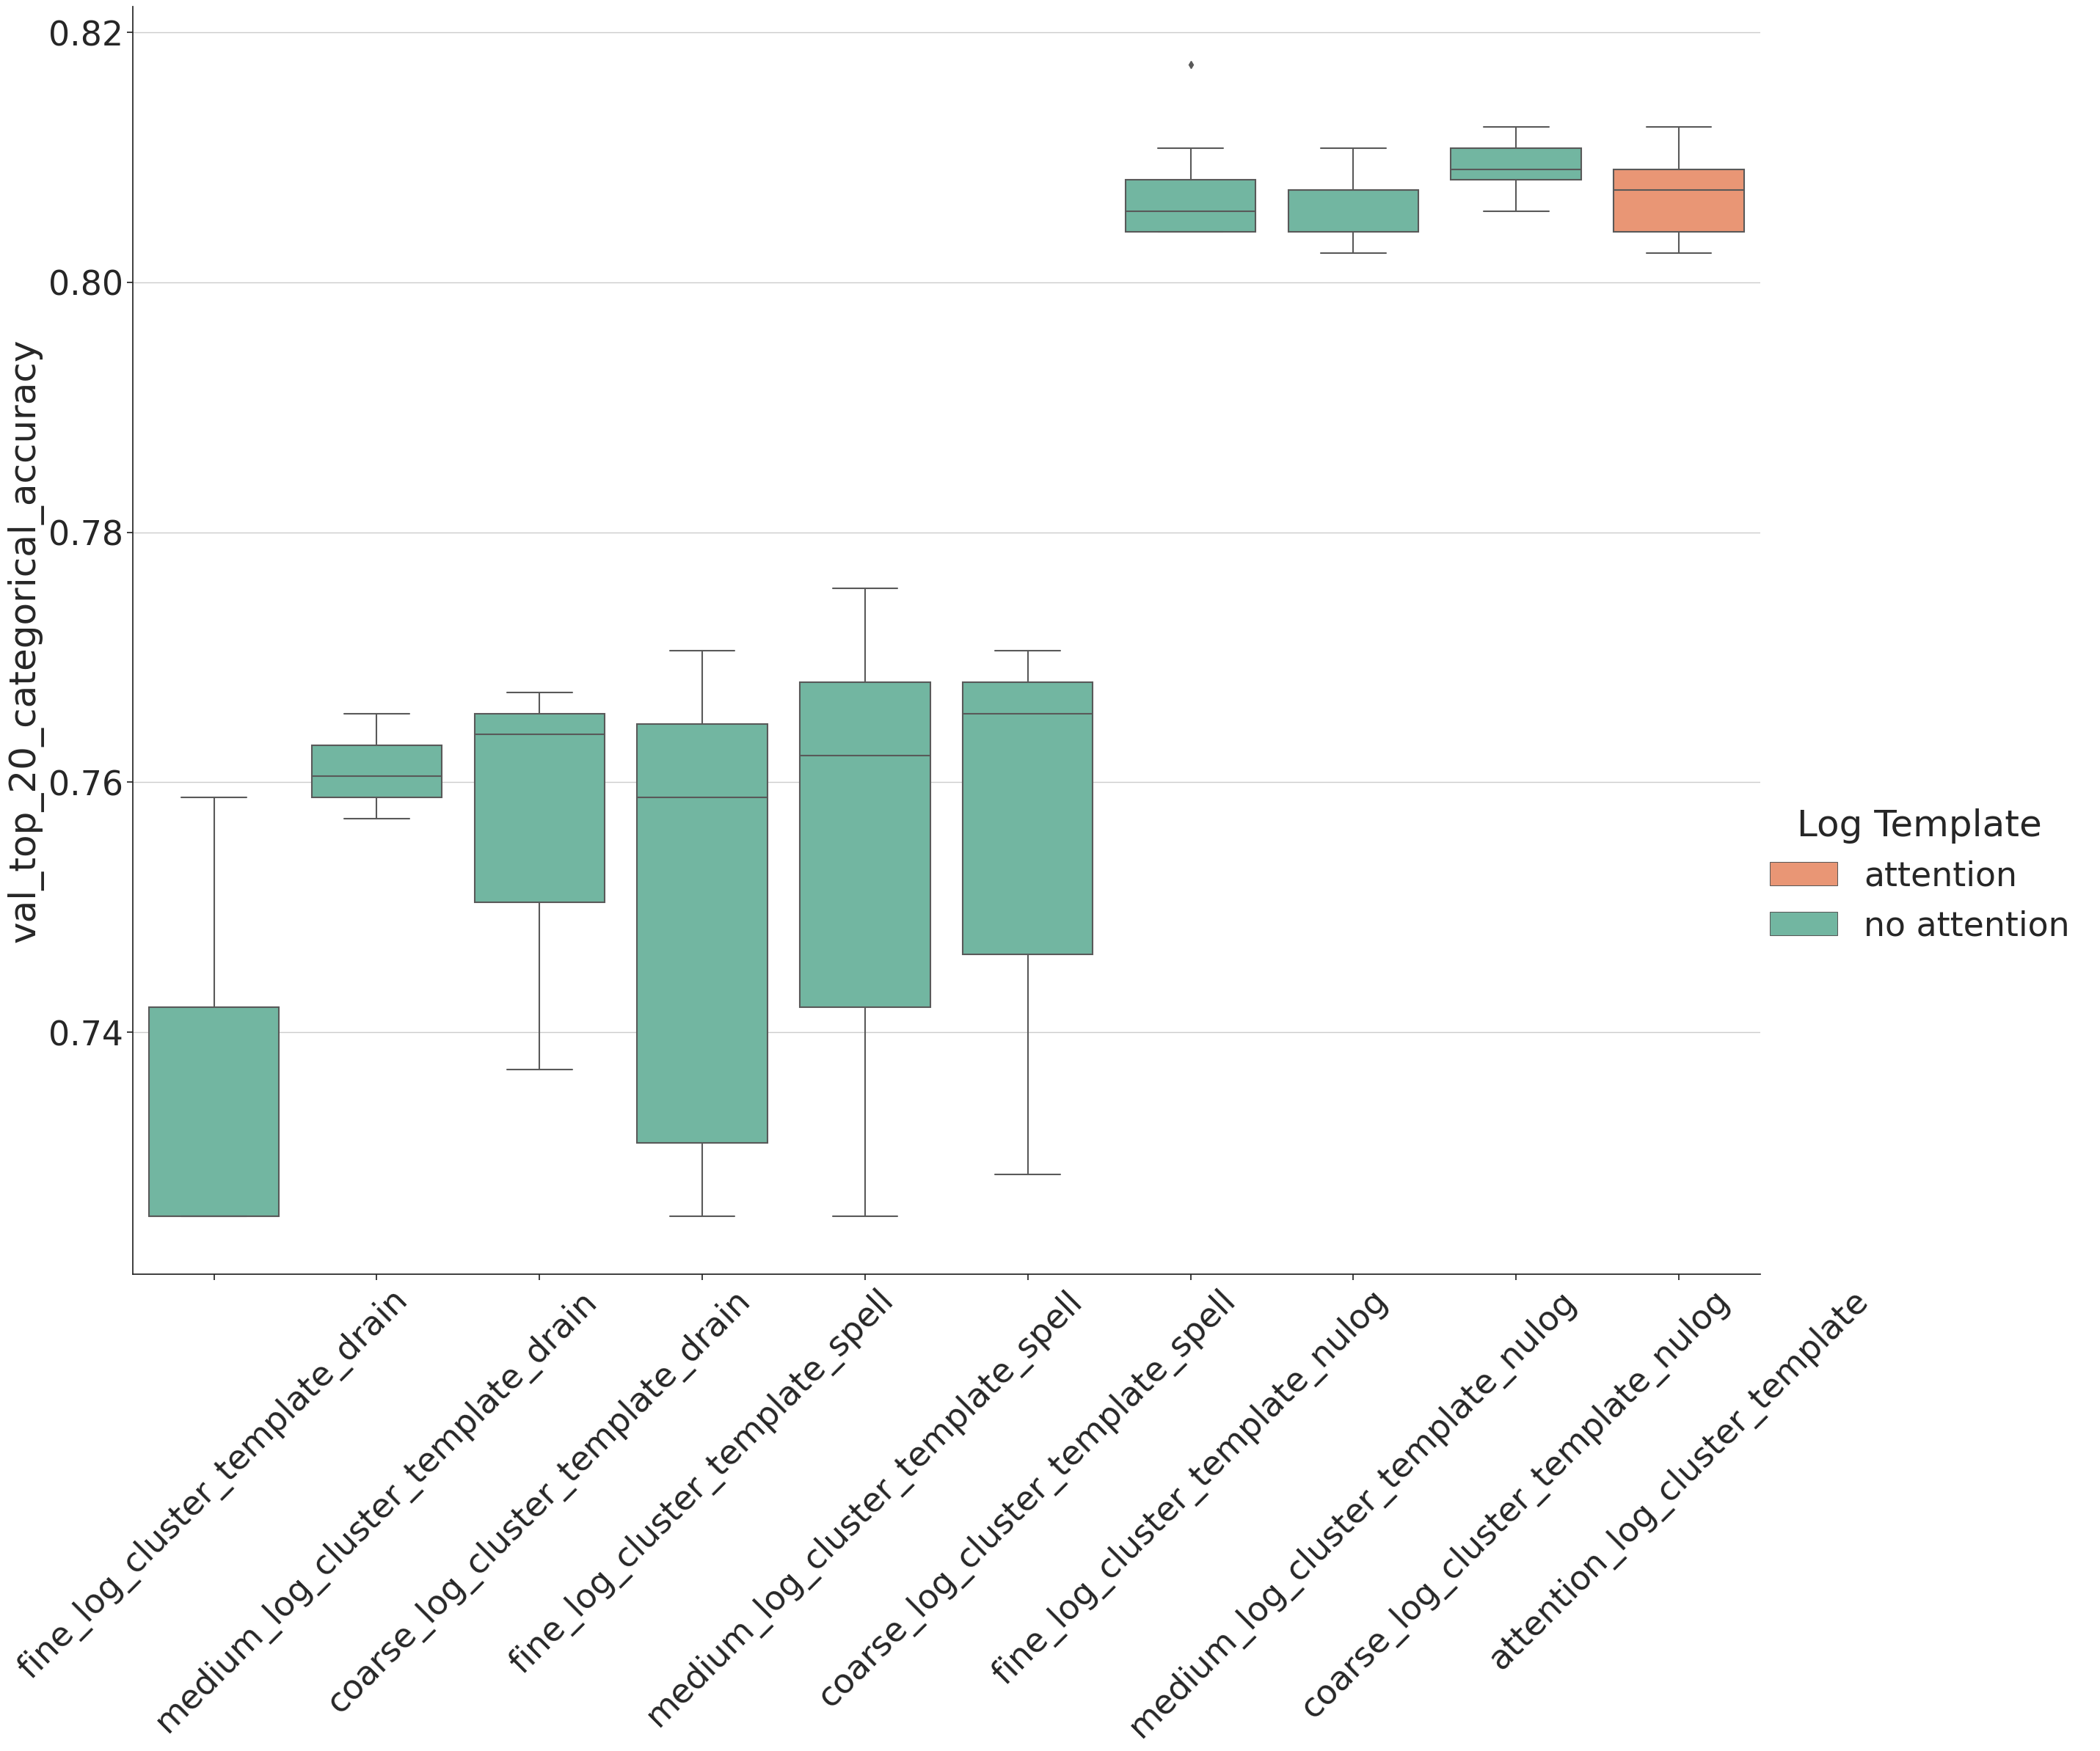
\includegraphics[keepaspectratio=true,scale=0.2]{figures/5_results/all_hdfs.png}
    \caption{Attention based selection from nine log templates generated by three log parsers with three parameterizations. Dataset size 2000 logs.}
    \label{fig:all_hdfs}
\end{figure}

Motivated by our earlier results that showed that using Drain and Spell performed better than combining all three algorithms [Figure \ref{fig:drain_spell}], we ran another experiment just with Nulog and Spell, because drain performed badly on this dataset. Contrary to the earlier experiment, we saw no improvement. 

\begin{figure}[H]
    \centering
    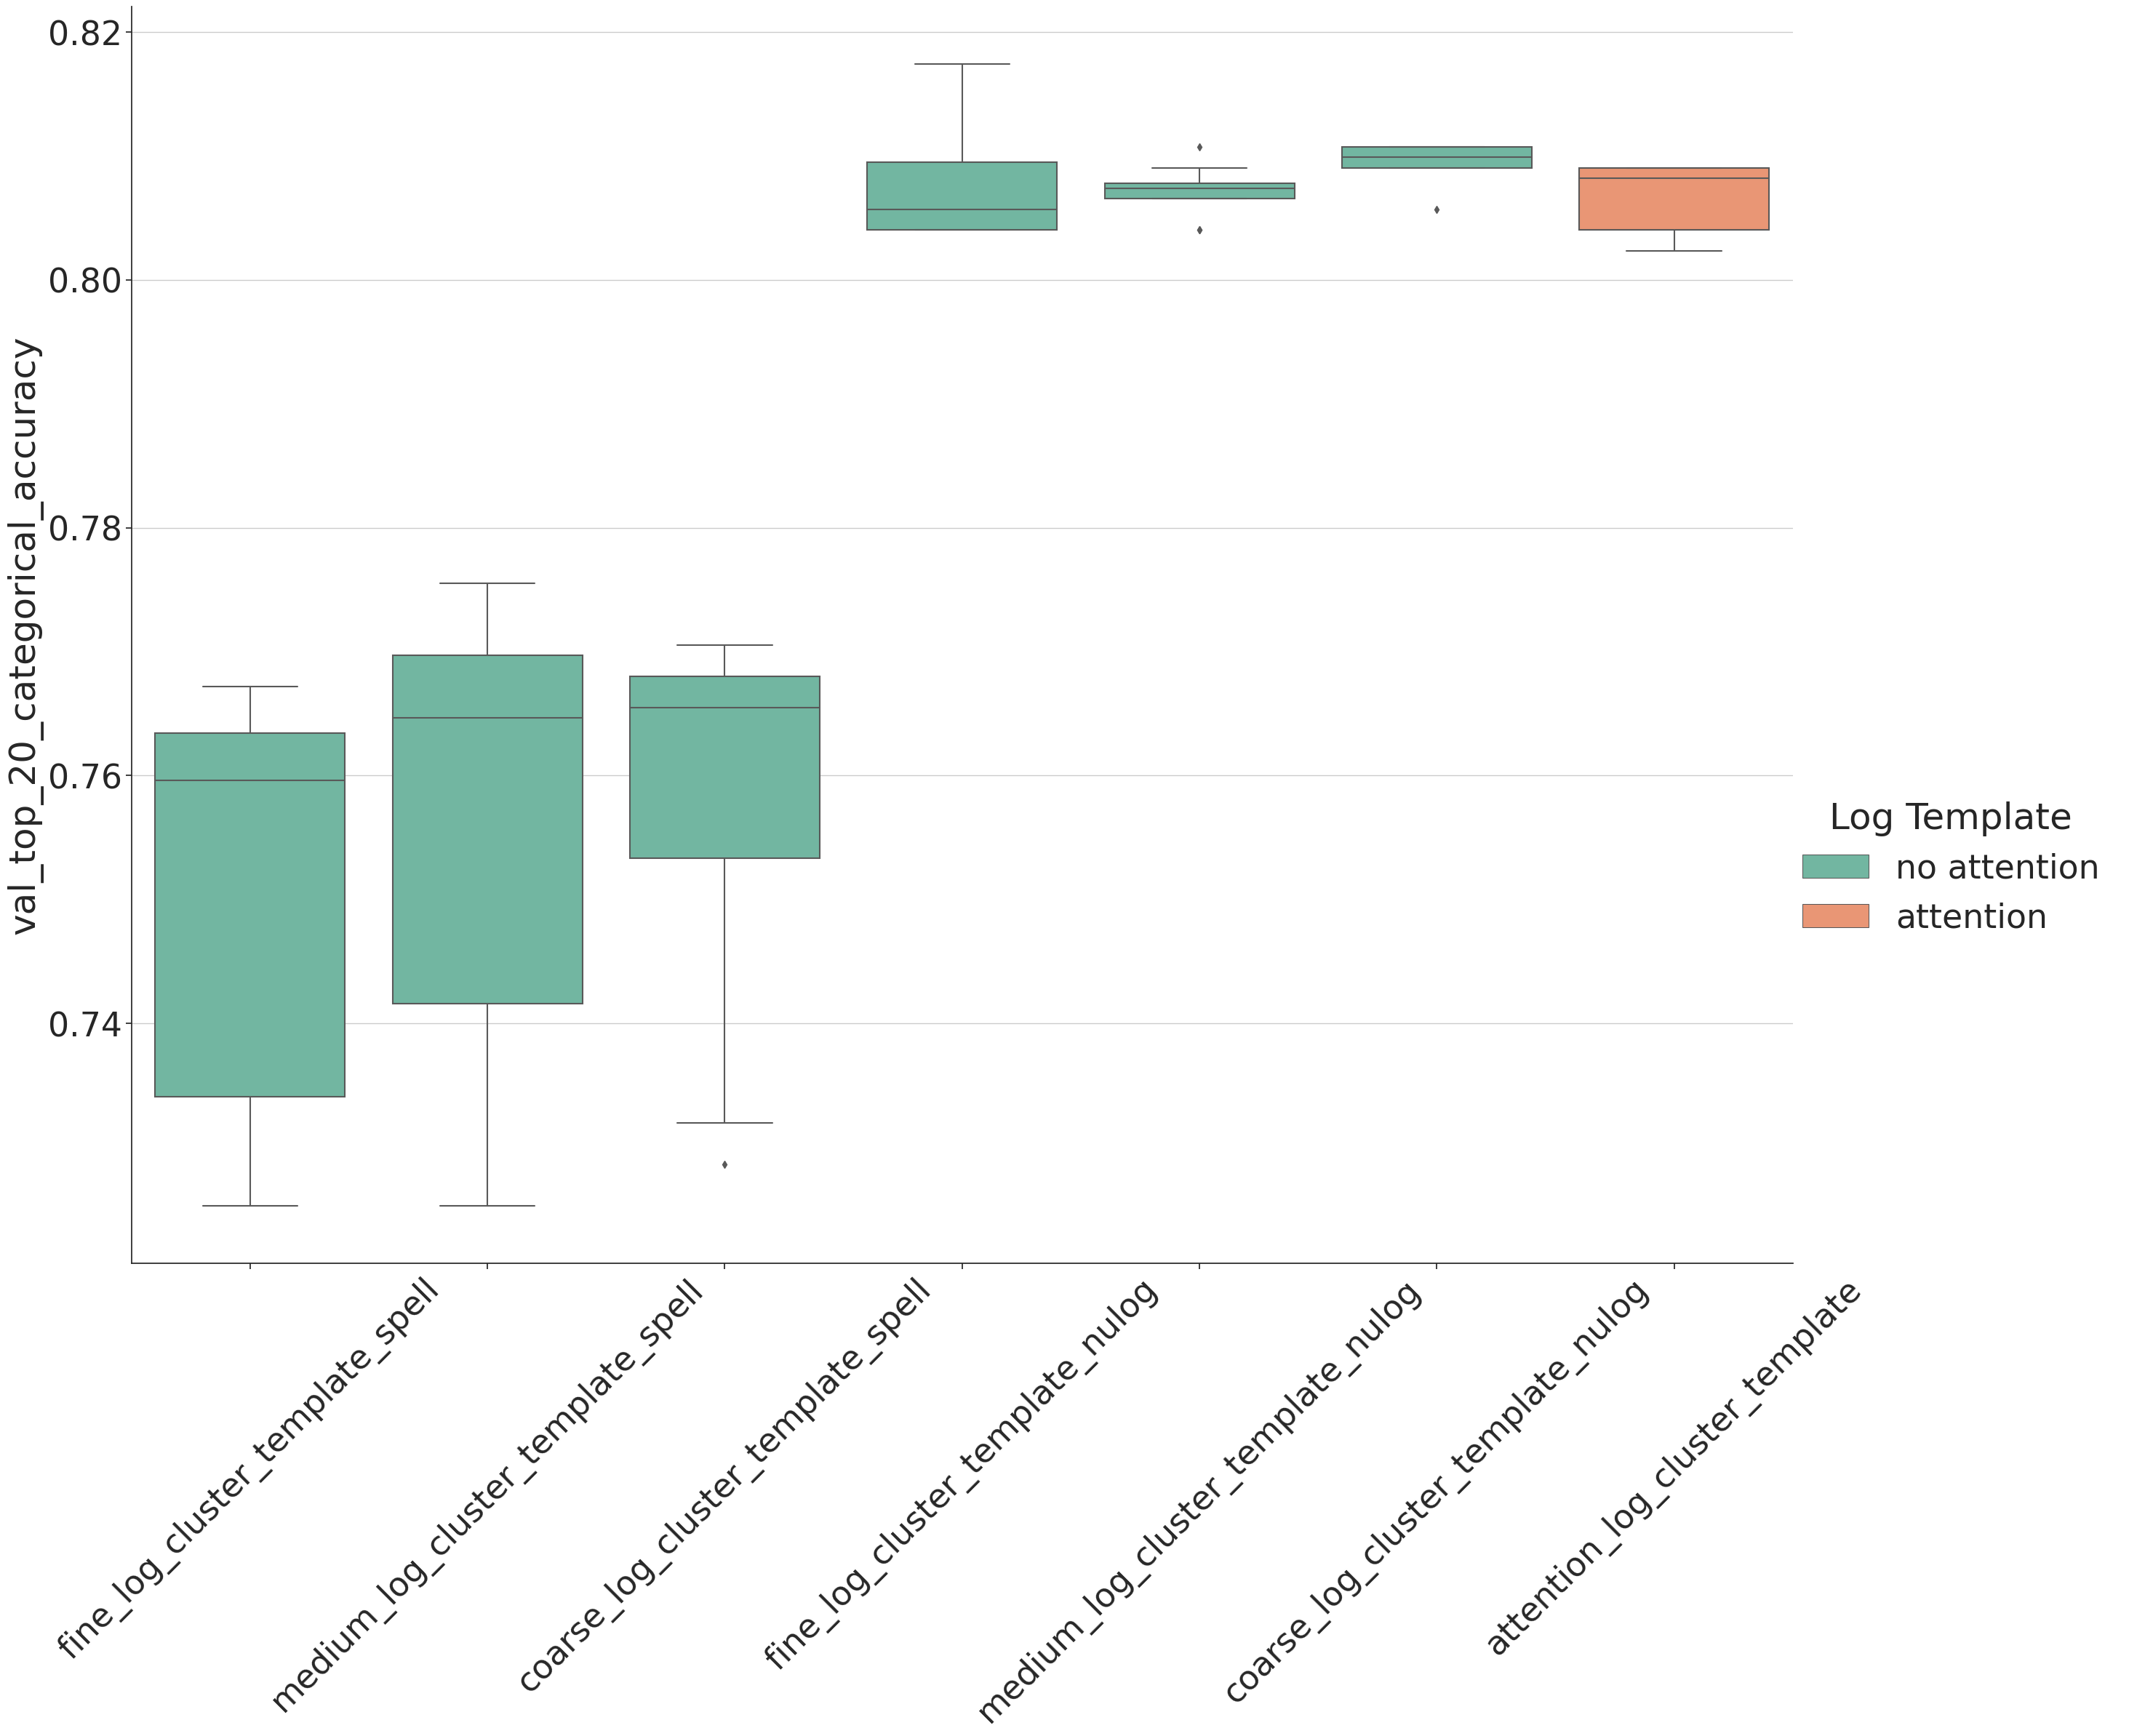
\includegraphics[keepaspectratio=true,scale=0.2]{figures/5_results/spell_nulog_hdfs.png}
    \caption{Attention based selection from six log templates generated by Spell and Nulog with three parameterizations. Dataset size 2000 logs.}
    \label{fig:spell_nulog_hdfs}
\end{figure}

\subsection{Thunderbird}
The results from our Thunderbird experiments differed the most from our original dataset. Drain produced by far the most templates, while the number of templates was generally already much higher than for the other datasets. Using drain templates alone also led to the highest experiment runtime, longer even than when using the combination of all templates. During our Drain and Spell experiments, the model also stopped learning very early and did not improve its validation accuracy beyond the initial value. 

\begin{table}[htbp]
  \centering
  \begin{tabular}{cccc}
    \hline
    \textbf{Parser} & \textbf{No. of Templates} & \textbf{Runtime} & \textbf{Epochs learned} \\
    \hline
    Drain & 2661  & 12.1min & 6 \\
    Spell & 456   & 1.2min & 7 \\
    Nulog & 397  & 4.3min & 14 \\
    All & 3402 & 4.2min & 14 \\
    \hline
  \end{tabular}
  \caption{Number of log templates, epochs learned and runtime for different log parsers. Thunderbird logs. }
  \label{tab:thunderbird}
\end{table}

We can see in figure \ref{fig:all_tbird} several identical results for the prediction quality with no variance and generally very close, low values. 

\begin{figure}[H]
    \centering
    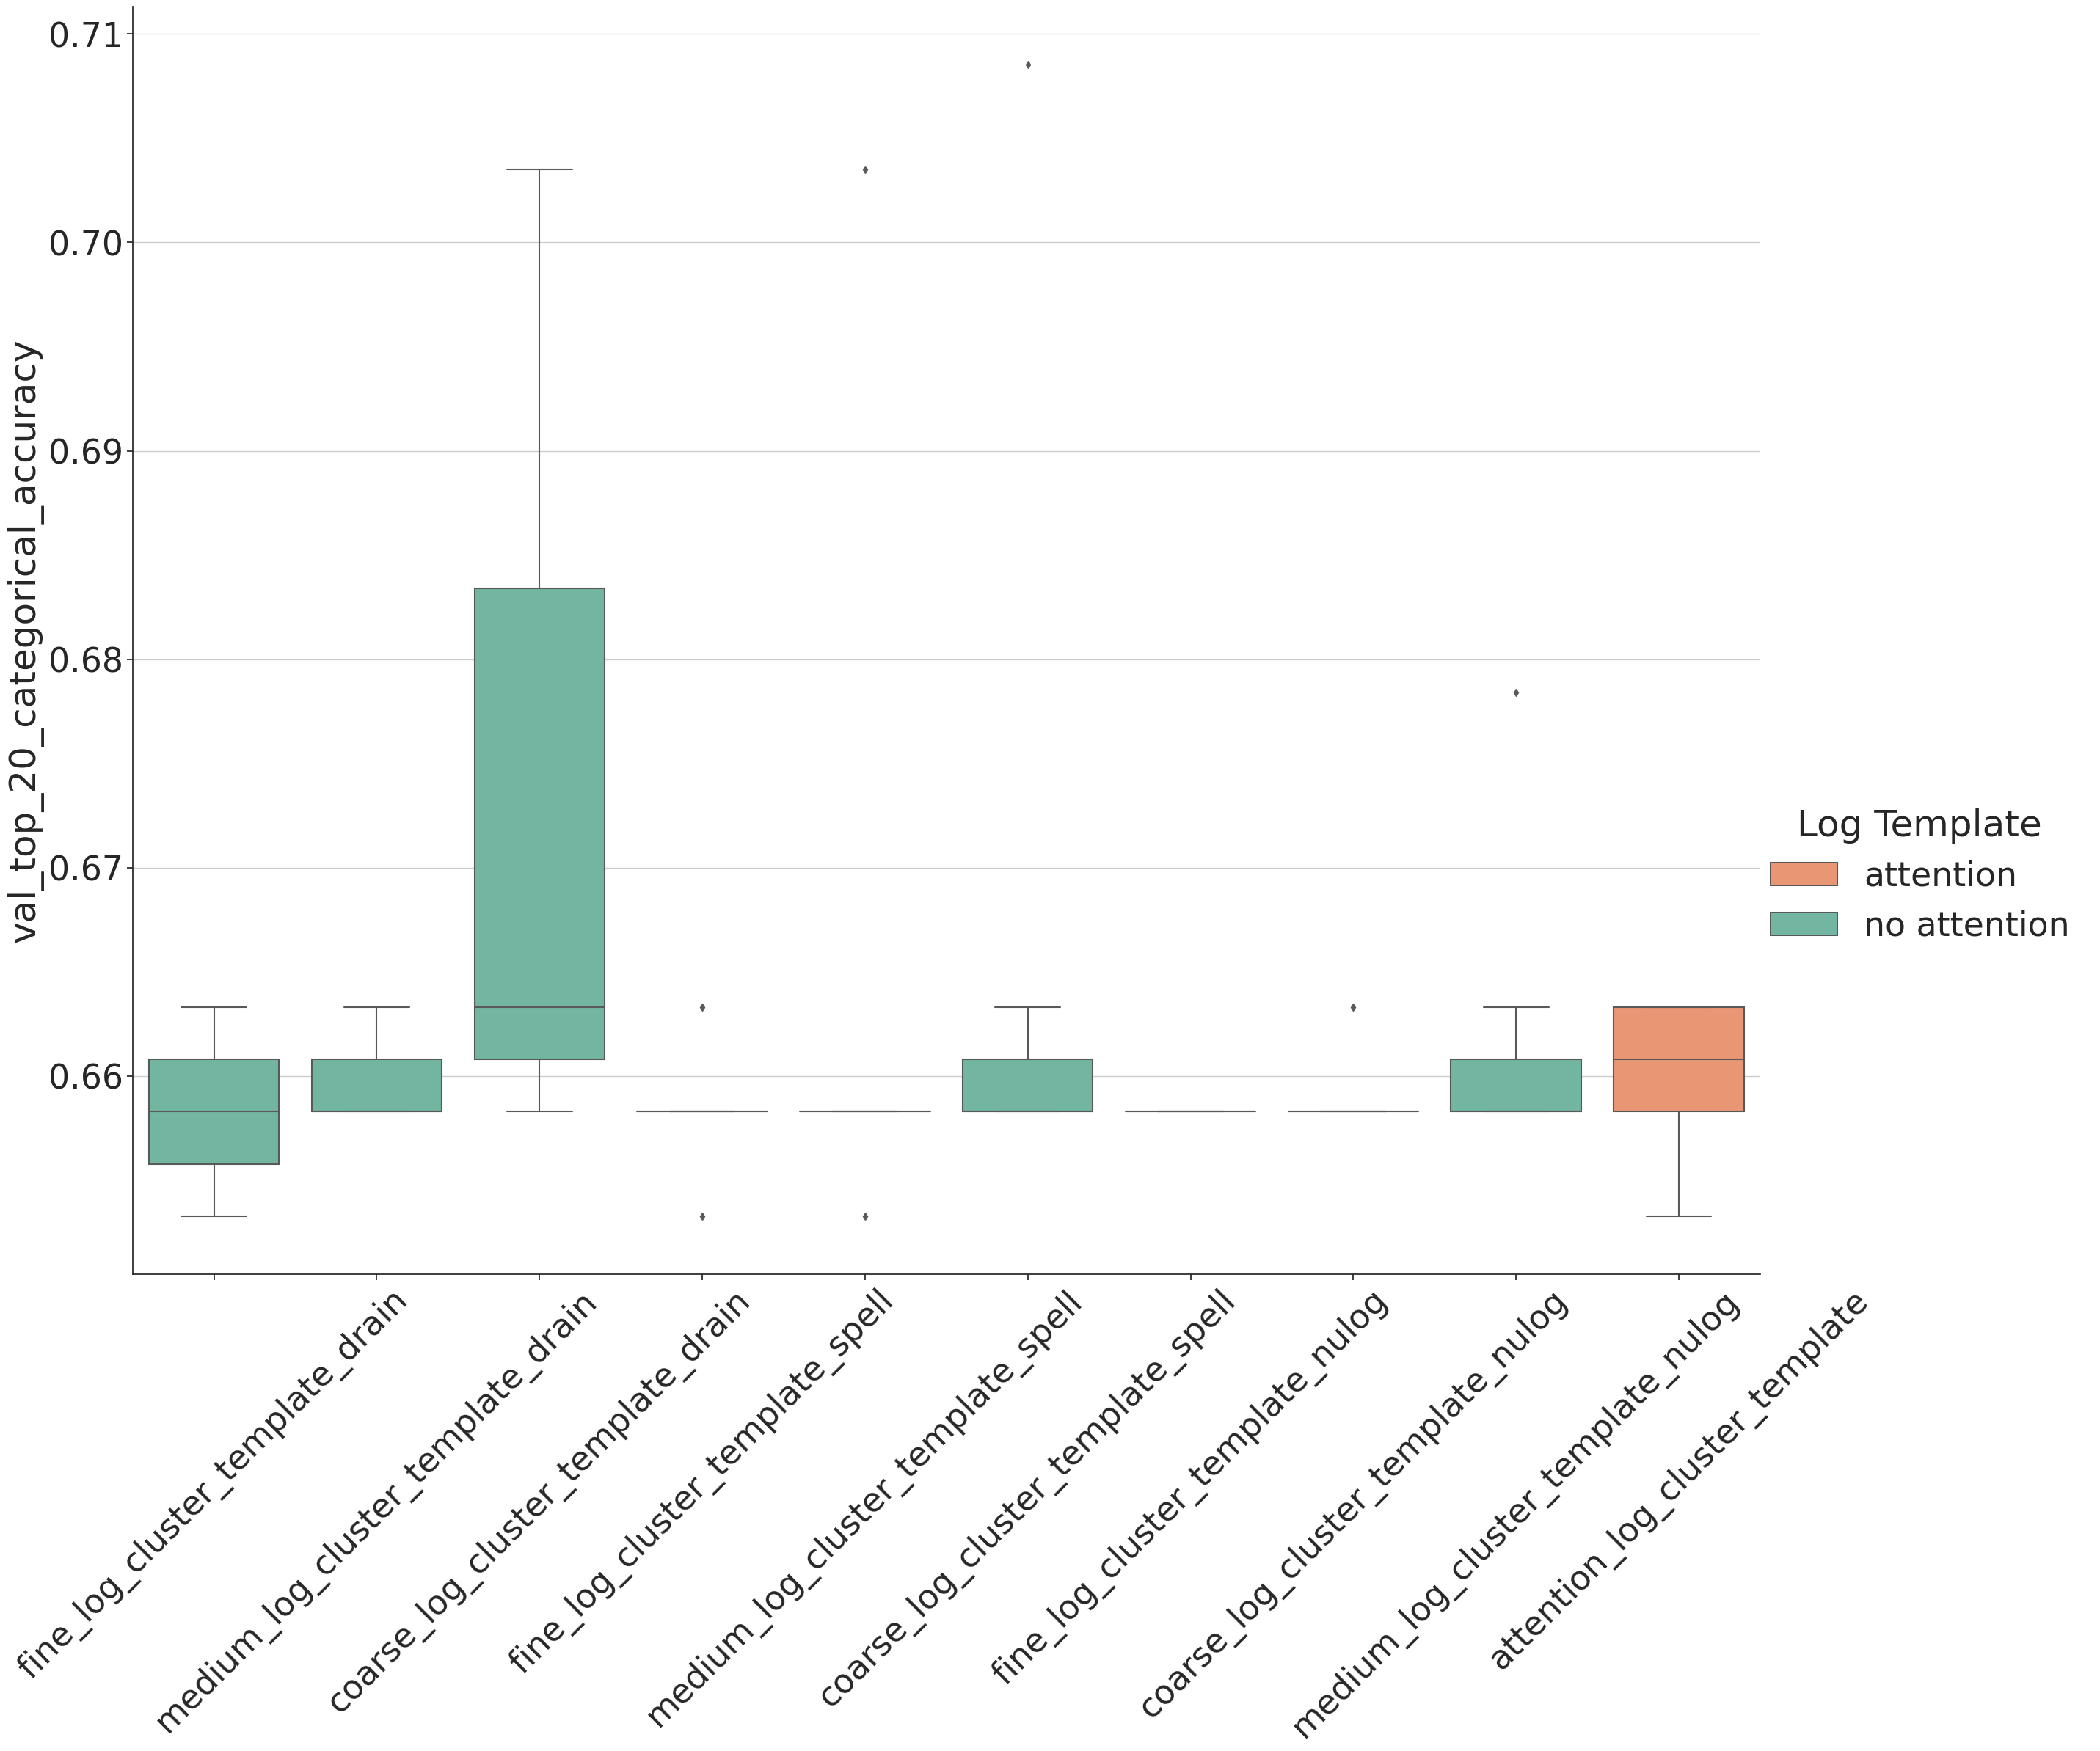
\includegraphics[keepaspectratio=true,scale=0.2]{figures/5_results/all_tbird.png}
    \caption{Attention based selection from nine log templates generated by three log parsers with three parameterizations. Dataset size 2000 logs.}
    \label{fig:all_tbird}
\end{figure}